\section{Smooth Line Connections}

While not required by the robot kinematics of the BeachBot (which can turn on the spot), generating smooth connections 
makes the developed algorithms generalizable for four-wheeled vehicles. Connecting the lines with curve that has the same tangent as the respective line is crucial to ensure a smooth driving process and to have the robot facing the right direction to continue the drawing.
It is also necessary to constrain the curvature for the path converter that translates the generated rake path into a robot path that is drivable by the bot. If the curvature at a given point of the connection is too high, it is not possible for the path converter to find a converging solution which makes tedious manual work needed to adjust the curvature of the connections until the converter is able to find a solution. The rounded connections also create a nice visual effect to spectators.

As conlusion, ideally a connection with upper limit on curvature\footnote{The curvature is defined as the inverse of the radius of the circle that the tangent produces at any given point in the curve. For a curve defined as $x(t)$ and $y(t)$, the curvature $\kappa$ is given by
\begin{equation}
\kappa = \frac{|x'y''-y'x''|}{(x'^2+y'^2)^{3/2}}
\end{equation}
} has to be found.

The connection curve parameters for any two elements can be chosen based on three variables, as shown in \autoref{fig:connections_vars}. $d$ is the distance between the two points (denoted by $a$ and $b$), $\alpha$ and $\beta$ are the angles defining the desired tangent to the connection curve at the start- respectively the endpoint.

\begin{figure}

\begin{figure}
\centering
\usetikzlibrary{calc}

\definecolor{cb3b3b3}{RGB}{179,179,179}
\definecolor{ccccccc}{RGB}{204,204,204}
\definecolor{cffffff}{RGB}{255,255,255}

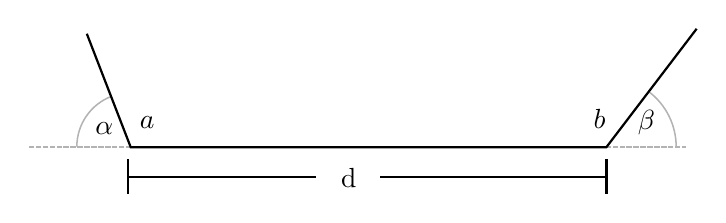
\begin{tikzpicture}[y=0.80pt,x=0.80pt,yscale=-1, inner sep=0pt, outer sep=0pt]
\centering

  \path[draw=cb3b3b3,dash pattern=on 2pt off 0.5pt,line join=miter,line
    cap=butt,miter limit=4.00,dash phase=0.201pt,line width=0.800pt]
    (115.9129,172.6241) -- (69.8665,172.6241);
  \path[draw=cb3b3b3,dash pattern=on 2pt off 0.5pt,line join=miter,line
    cap=butt,miter limit=4.00,dash phase=0.201pt,line width=0.800pt]
    (330.6888,172.6195) -- (366.5496,172.6195);
  \path[cm={{1.45393,0.0,0.0,1.45393,(-471.01666,-377.22731)}},draw=cb3b3b3,miter
    limit=4.00,line width=0.550pt] (564.5997,360.8878)arc(-52.961:0.593:21.466);
  \path[cm={{0.52395,0.0,0.0,0.52395,(41.81533,-25.47312)}},draw=cb3b3b3,miter
    limit=4.00,dash phase=8pt,line width=0.55pt]
    (94.9543,377.5908)arc(179.987:249.624:46.467);
  \path[fill=black,line width=0.800pt] (100,167) node[above right]
    (text4046) {$\alpha$};
  \path[fill=black] (345,167) node[above right] (text4046-2)
    {$\beta$};
  \path[draw=black,line join=miter,line cap=butt,line width=0.800pt]
    (114.8543,177.9195) -- (114.8543,193.7975);
  \path[draw=black,line join=miter,line cap=butt,line width=0.800pt]
    (114.8543,186.1205) -- (330.7957,186.1205);
  \path[draw=black,line join=miter,line cap=butt,line width=0.800pt]
    (330.7957,177.9195) -- (330.7957,193.7975);
  \path[fill=cffffff,line width=0.800pt,rounded corners=0.0000cm]
    (199.5575,177.5072) rectangle (228.2820,192.5707);
  \path[fill=black,line width=0.800pt] (211,191) node[above right]
    (text4081) {d};
  \path[draw=black,line join=miter,line cap=butt,line width=0.800pt]
    (96.0814,121.3474) -- (115.9166,172.6195) -- (330.7355,172.6195) --
    (371.5287,119.1019);
      \path[] (120,164) node[above right]
    (text4046) {$a$};
      \path[] (325,164) node[above right]
    (text4047) {$b$};
\end{tikzpicture}
\caption{Variables for the connection between two elements at points $a$ and $b$: tangents $\alpha$ and $\beta$ and distance $d$}
\label{fig:connections_vars}
\end{figure}


\label{fig:connections_vars}
\end{figure}


\subsubsection{Beziér Splines}

\begin{figure}
\centering
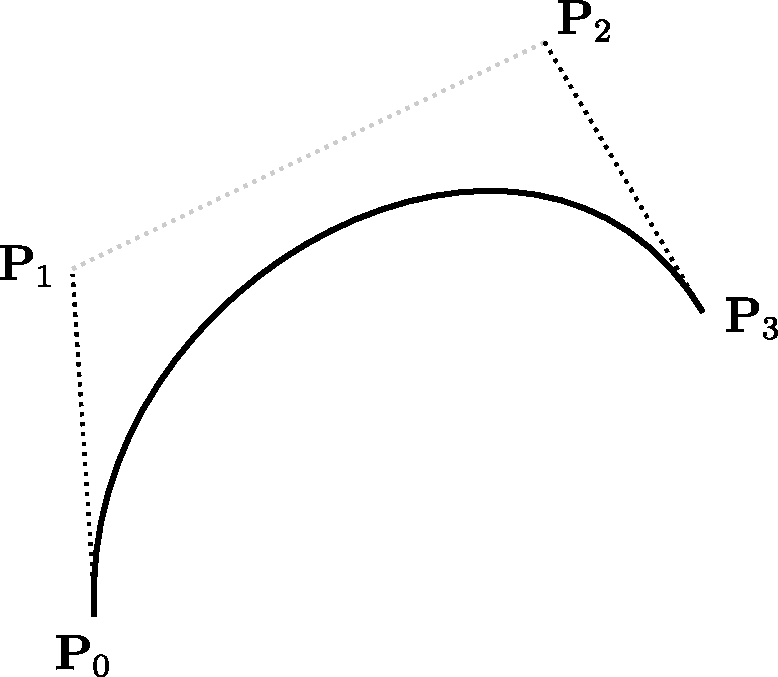
\includegraphics[width=0.7\textwidth]{images/smooth/bezier_3rd.pdf}
\caption{A bezier curve of 3rd degree with the control points $P_0 \ldots P_3$.}
\label{fig:bez_3rd}
\end{figure}

A first approach to generate curved connections between elements was by using Beziér splines. Beziér splines are commonly utilized in many computer graphics programs as vector graphics editors or computer aided design applications. They are based on Bernstein polynomials and defined as follows: given a set of control points $P_0, P_1 \ldots P_n$ and $t \in \left[ 0, 1\right]$, the Beziér curve is, in its explicit form, given by:

\begin{equation}
\mathbf{B}(t) = \sum_{i=0}^n {n\choose i}(1 - t)^{n - i}t^i\mathbf{P}_i
\end{equation}

(${n\choose i}$ are the binomial coefficients).

Expanding the Bernstein polynomials for the third order Beziér curve yields:

\begin{equation}
\mathbf{B}(t)=(1-t)^3\mathbf{P}_0+3(1-t)^2t\mathbf{P}_1+3(1-t)t^2\mathbf{P}_2+t^3\mathbf{P}_3 \mbox{ , } t \in [0,1]
\end{equation}

or the fifth order:

\begin{equation}
\begin{split}
\mathbf{B}(t) = (1 - t)^5\mathbf{P}_0 & + 5t(1 - t)^4\mathbf{P}_1 + 10t^2(1 - t)^3 \mathbf{P}_2 \\ 
& +  10t^3 (1-t)^2 \mathbf{P}_3 + 5t^4(1-t) \mathbf{P}_4 + t^5 \mathbf{P}_5 \mbox{ , } t \in [0,1]
\end{split}
\label{bez_quint}
\end{equation}

As first approach, Beziér splines of 3rd order were used. $P_0$ and $P_n$ (in this case $n=3$) of the Beziér spline are trivially found as the start- and endpoint of the connection.  Beziér splines of 3rd order only have 2 free control points, which can, by moving them along the tangent defined by $\alpha$ and $\beta$, easily be used to create a connection that connects smoothly in the start and endpoint. However, the curvature for the complete curve can not be defined because the two control points offer to few degrees of freedom. A beziér curve of 5th degree (quintic) has enough degrees of freedom to constrain the connection in terms of curvature.

The quintic Beziér curve consists of 6 control points $P_0 \ldots P_5$ that define the shape of the curve (\autoref{bez_quint}). $P_0$ and $P_5$ are again trivially chosen because they coincide with the start- respectively the endpoint of the curves that should be connected. $P_1$ and $P_4$ are also easy to choose as they have to be positioned on the tangents of the curves that should be connected. $P_2$ and $P_3$ on the other hand are more difficult to obtain. Even after an extensive search through available literature no analytical solution to this problem was found and it is likely that there is none, since the equation for curvature is getting quite complicated if expanded. In \cite{doi:10.1137/1.9781611971521.ch5} three approaches to generate Beziér splines with monotone curvature are discussed. \cite{choi2010piecewise} uses piecewise 3rd degree bezier curves to create a curvature and corridor constrained trajectory.

\begin{figure}
\centering
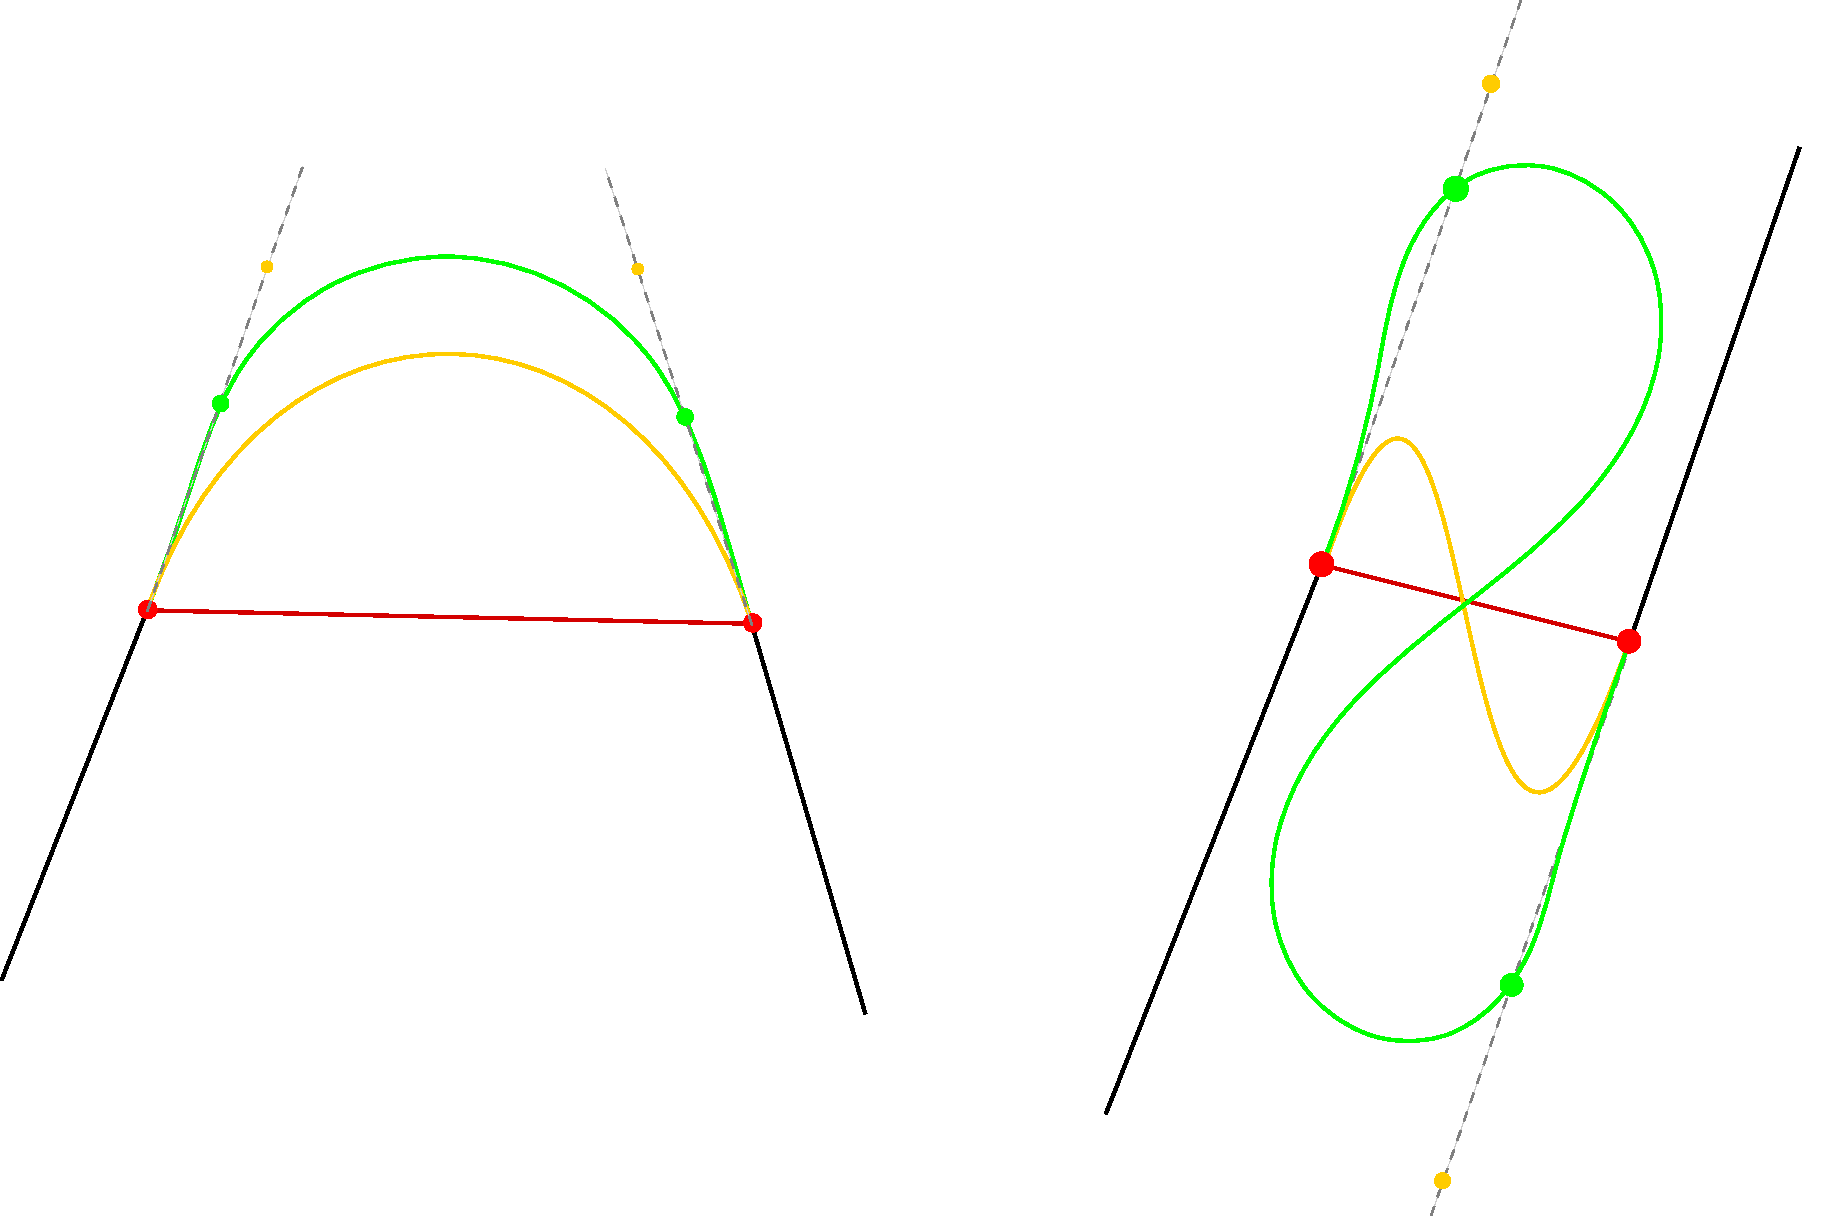
\includegraphics[width=0.8\textwidth]{images/smooth/spiro_connect_comparison.pdf}
\caption{Comparison between connection types: dashed gray indicates the tangent to the elements that should be connected (black). The red line is the straight connection. In yellow, the connection by using Beziér curves of third degree is shown, with the control points also in yellow. The green line shows what a connection with two spiro control points looks like.}\label{fig:comp_bez_spiro}
\end{figure}

\subsubsection{Spiro Splines}\label{sec:smoothspiro}

Spiro splines, introduced by R. Levien \cite{levien2009spiral} are a different approach specifically created for the purpose of designing fair curves. The main scope of application is the design of typefaces. 

They have several properties which make them well-suited for the task at hand.

Five different control points can be utilized to control the shape of the curve. In contrast to Beziér curves, the calculated curve is always passing through all of the control points, whereas the Beziér curve only passes through the first and last control point (also seen in the comparison in \autoref{fig:comp_bez_spiro}). The five different control points, denoted by a single character, of spiro splines are as follows:

\begin{itemize}
\item[\texttt{v}] Corner point
\item[\texttt{c}] A $G^2$ continous constraint. The curvature  on the left side is the same as on the right side ($\kappa_l = \kappa_r$).
\item[\texttt{o}] Similiar to \texttt{c}, a $G^4$ continous constraint. Not only $\kappa_l = \kappa_r$ is true, but also the first and second derivative of the curvature is constrained ($\kappa_l' = \kappa_r'$, $\kappa_l'' = \kappa_r''$).
\item[\texttt{[}] A straight-to-curved control point that acts like a tangent constraint in this case.
\item[\texttt{]}] A curved-to-straight control point that also acts like a tangent constraint here.
\end{itemize}

In this thesis, the $G^4$ control point remains unused. This has two reasons: First, a $G^4$ continuity is not needed for the purpose of generating a smooth robot trajectory and second, the $G^4$ control point is not as numerically stable as the $G^2$ control point and is therefore less tolerant to arbitrary placement.

The interpolation curve between the control points is calculated by cutting appropriate parts from the Euler-Spiral (or Cornu curve) by a numerical method. The Euler-Spiral, shown in \autoref{euler_spiral}, is a well-known example for a clothoid, a family of curves where the curvature changes linearly over the arc length). % The Euler-Spiral is intrinsically described by $\kappa(s) = s/2$.

A plot over a wide range of possible values for $\alpha$ and $\beta$ is shown in \autoref{spiro_param}.

\begin{figure}
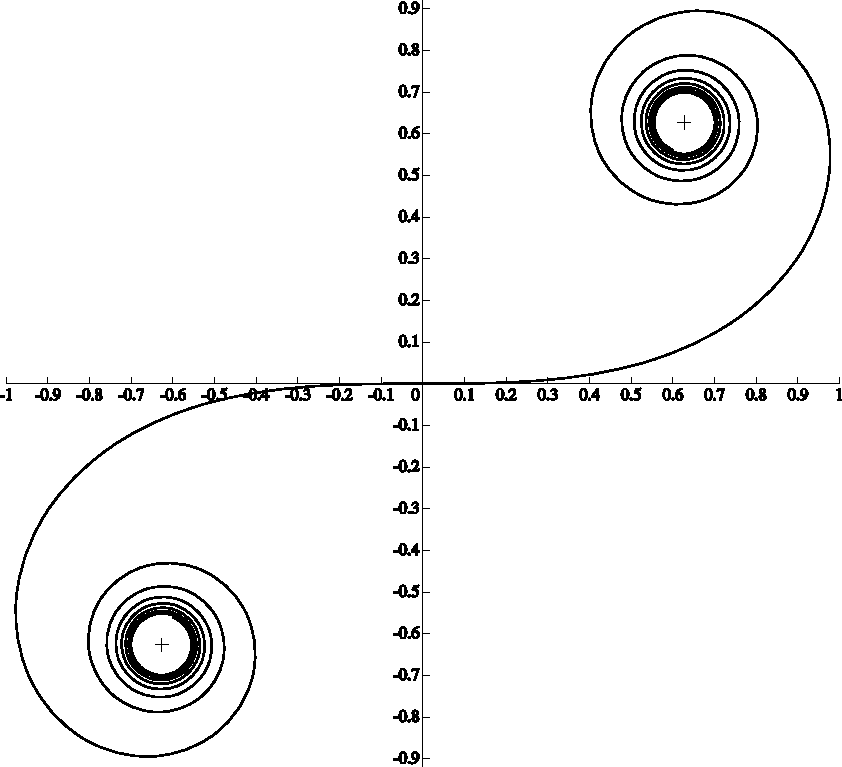
\includegraphics[width=\textwidth]{images/smooth/euler_spiral.pdf}
\caption{The Euler spiral (plot taken from \cite{levien2009spiral}, p. 49)}
\end{figure}

\begin{figure}
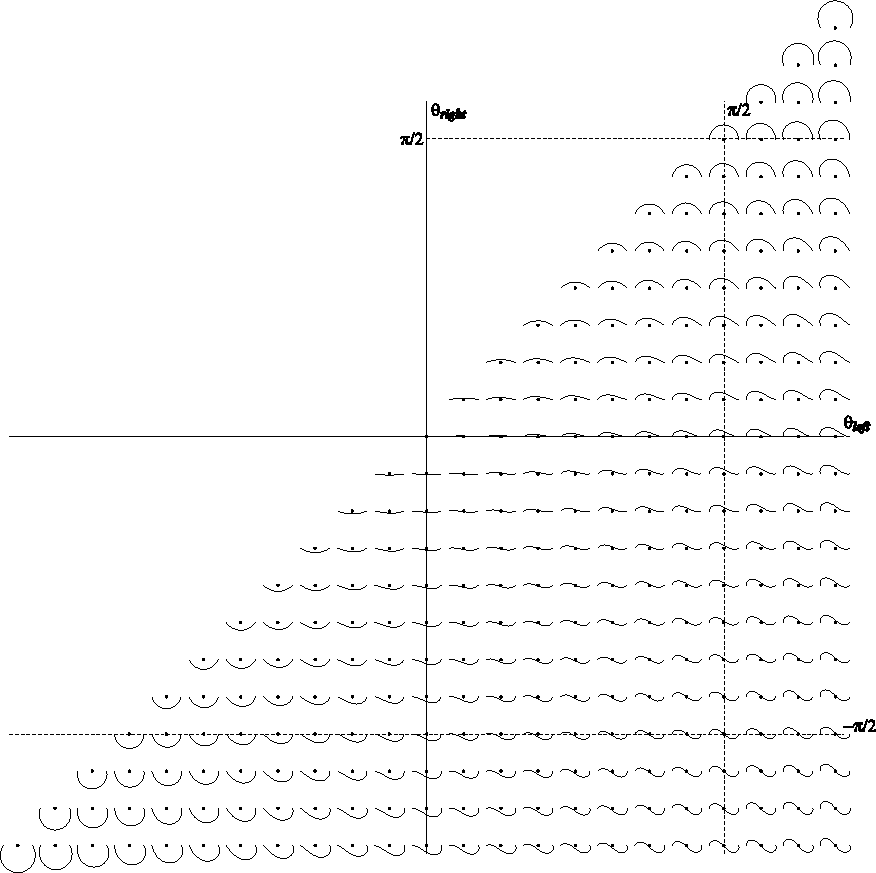
\includegraphics[width=\textwidth]{images/smooth/euler_spline_primitive.pdf}
\caption{The spline based on the Euler spiral plotted over the parameter space (plot taken from \cite{levien2009spiral}, p. 50)}\label{spiro_param}
\end{figure}

%If $G^2$ or $G^4$ constraints are used, the curve can not unsmooth (compare \autoref{fig:unsmooth}).

%\begin{figure}
%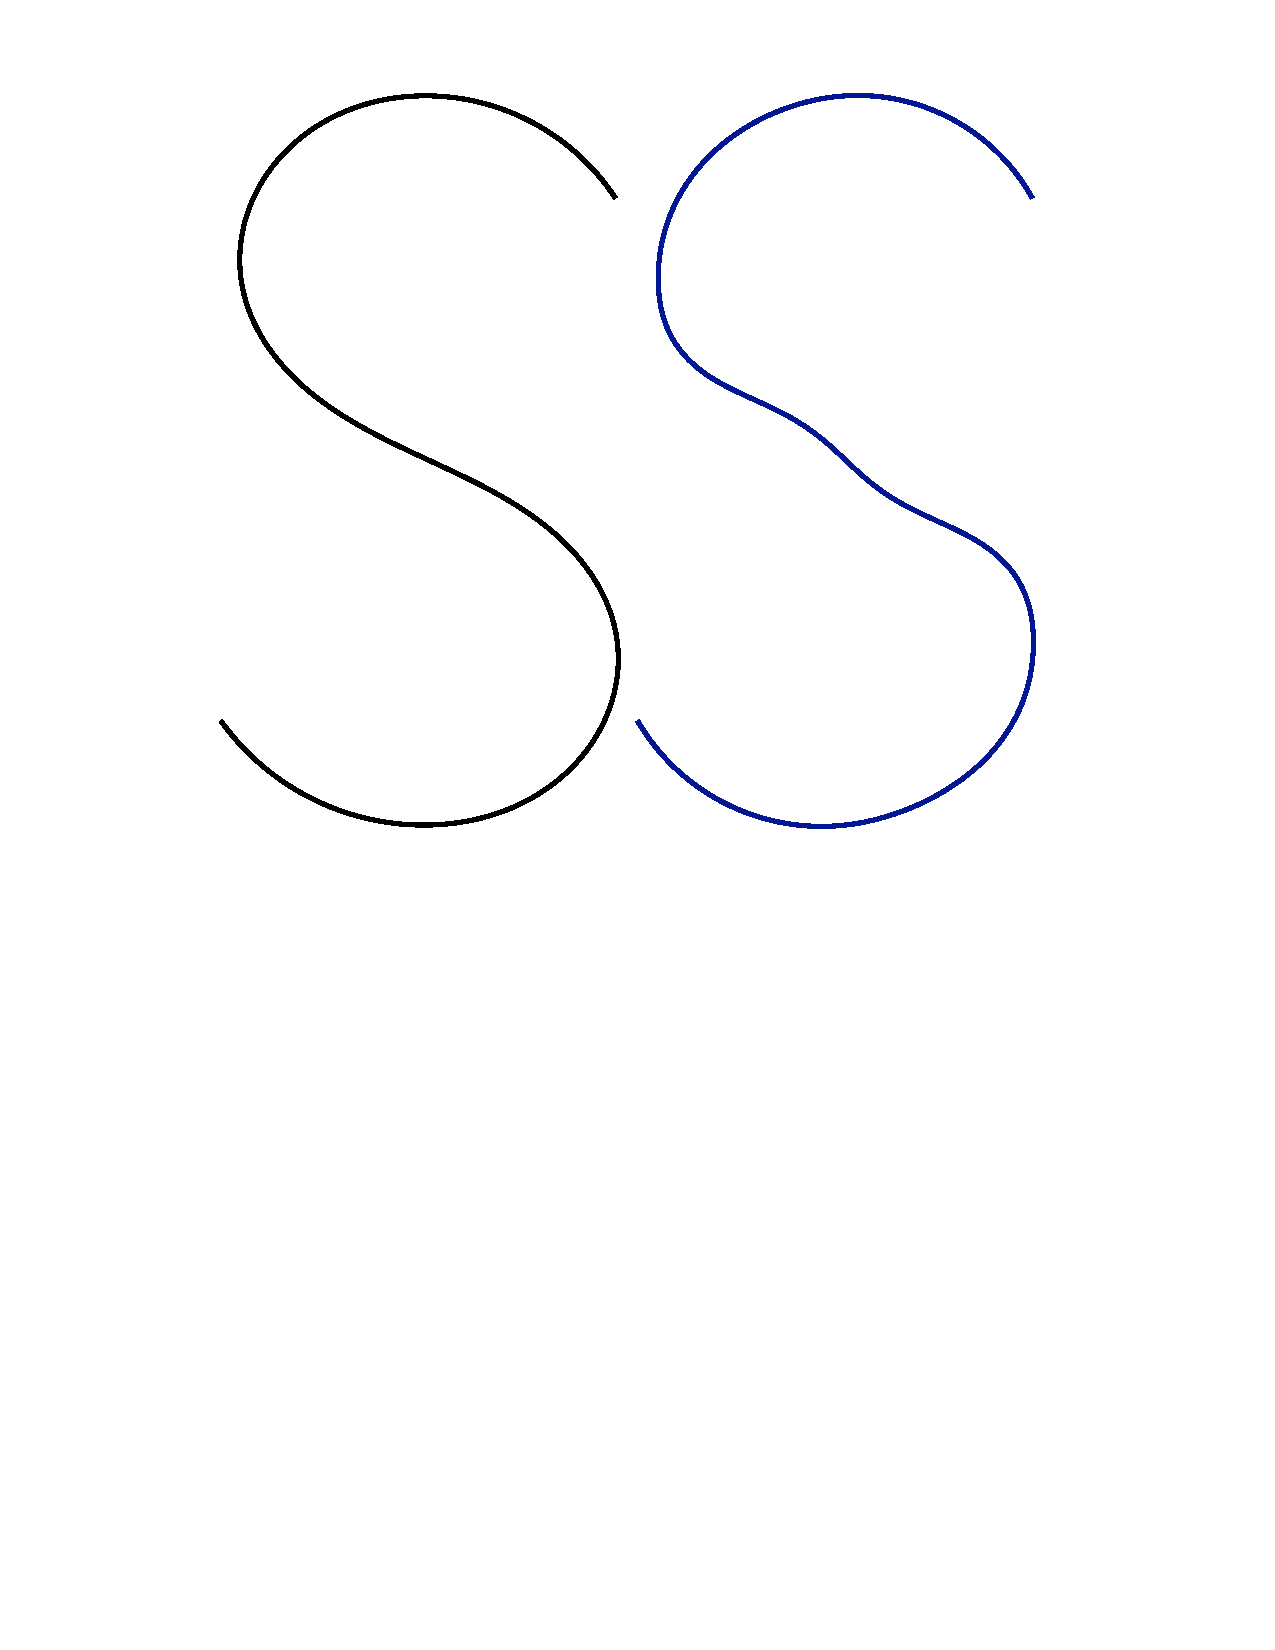
\includegraphics[width=\textwidth]{images/smooth/continuity.pdf}
%\caption{A curve created with spiro points with $G^2$ or $G^4$ continuity can never be unsmooth (like the right %\enquote{S} shape). Figure taken from \cite{levien2009spiral}}\label{fig:unsmooth}
%\end{figure}

The author, Raph Levien, has published his reference implementation \footnote{libspiro: \url{http://www.levien.com/spiro/}} of spiro splines as free software, which makes it possible to be used by this thesis. The implementation is fast enough to even allow for realtime editing. That guarantees that the curve generation would not be the bottleneck of the application in terms of time consumption. The input to the library is a sequence of the control points with coordinates attachend and the output is discretized to a set of Beziér curves which are more common for drawing and editing in graphics programs.

\paragraph{Heuristic for Setting the Control Points}

To find suitable locations for the spiro spline control points, a heuristic was used.

All connection constraints can be expressed by 5 variables: Connection length ($d$), tangents with angles $\alpha$ and $\beta$ and the curvature limit $\kappa$, as shown in \autoref{fig:connection_vars}. For the calculation of the control points, the difference between the two angles was defined as $\delta = \alpha - \beta$. It equals the angle between the two tangent vectors. 

Finding the first 4 points of the curve is straightforward: the first control point is a corner point at the endpoint of the first element. The second point is a straight-to-curve point, that is positioned an infinitesimally small distance in the direction of the tangent from the first point. This constrains the \enquote{outgoing} tangent. Vice versa, the same control points are set at the end of the curve, where the element that is connected to begins. Thus both tangent constrains are fullfilled. Because the spiros do not offer a direct way of setting the maximum and minimum curvatures, zero to two more control points have to be added. The curvature can be limited by positioning a $G^2$ control point at distance $2 * R$ from the start- and endpoint (as demonstrated in \autoref{fig:comp_bez_spiro}). This limits the curvature to the left and to the right of the control point to be the same. Since the highest curvature between the startpoint and the $G^2$ point would be a circular arc with radius $R$ (compare \autoref{spiro_param}) this limits the curvature to $\kappa = 1/R$, as long as both $G^2$ points are keeping a distance of $2*R$ as well.

The heuristic differentiates 3 cases:

If both tangent vectors $\alpha$ and $\beta$ point into a similar direction %and the circle that is described by them and $d$ has a radius that is in the range of $R < r < 2*R$ 
then no intermediate $G^2$ points are set because the connection will already be smooth and optimal.

Otherwise, the $G^2$ points, called $c_1$ and $c_2$ from hereon, are set by elongating the tangent vector to $2*R$ and placing the points at the resulting coordinate.
% and rotating it by $0.5 * \alpha$. This is done to reduce the size of the resulting curve, which is demonstrated in .. Fig ...

As discussed, the two $G^2$ points, called $c_1$ and $c_2$ are closer than $2 * R$ to each other, the positions have to be recalculated. This happens by rotating the $c_1$ and $c_2$ points gradually in different direction until positions are found that conform to the distance constraint. By rotating both points about the same angle, a symmetry is kept.

If both tangent vectors are showing in opposite directions and are on the same side of the straight connection line (compare \autoref{fig:conn_infty}), the resulting arc stretches to infinity if the angle between of the tangents and the connection line become very small. To counter this, $c_1$ and $c_2$ are rotated by $0.5 * (\pi - \alpha)$ and $0.5 * (\pi - \beta)$ respectively, if, as stated both tangent vectors are on the same side and both $\alpha$ and $\beta$ are smaller than $\pi/2$. The resulting curve is illustrated in \autoref{fig:conn_infty_rot}.

\begin{figure}
\centering
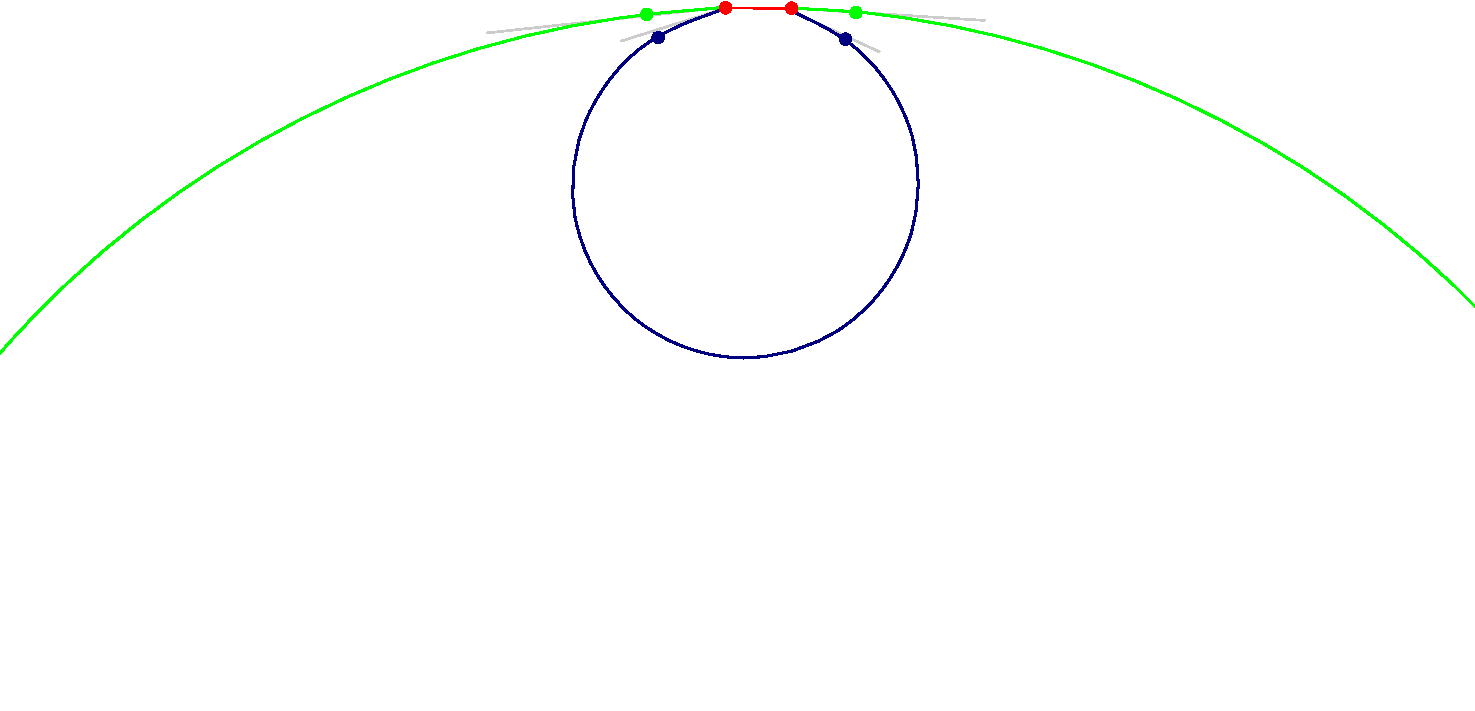
\includegraphics[width=0.8\textwidth]{images/smooth/tangents_infinity.pdf}
\caption{If $\alpha$ and $\beta$ are small and tangent vectors are on the same side of the straight connection, the connnection becomes the circle defined by both tangents, which can stretch to infinity.}\label{fig:conn_infty}
\end{figure}	

\begin{figure}
\centering
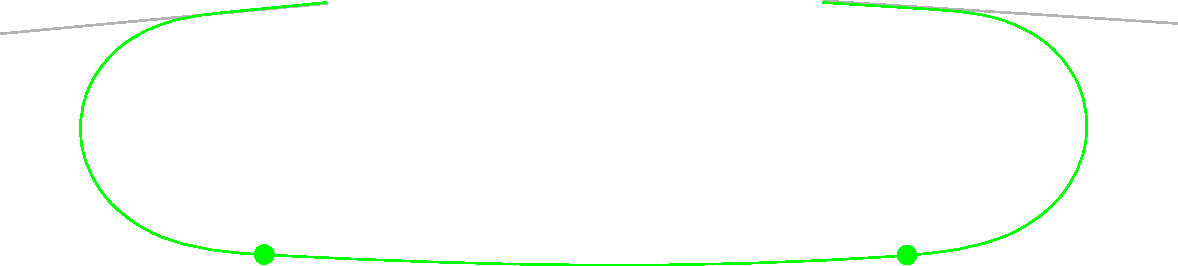
\includegraphics[width=0.8\textwidth]{images/smooth/tangents_infty_rotated.pdf}
\caption{Rotated control points produce a more favourable result for small $\alpha$ and $\beta$ values}\label{fig:conn_infty_rot}
\end{figure}	

\begin{figure}
\centering
\begin{subfigure}[b]{0.8\textwidth}
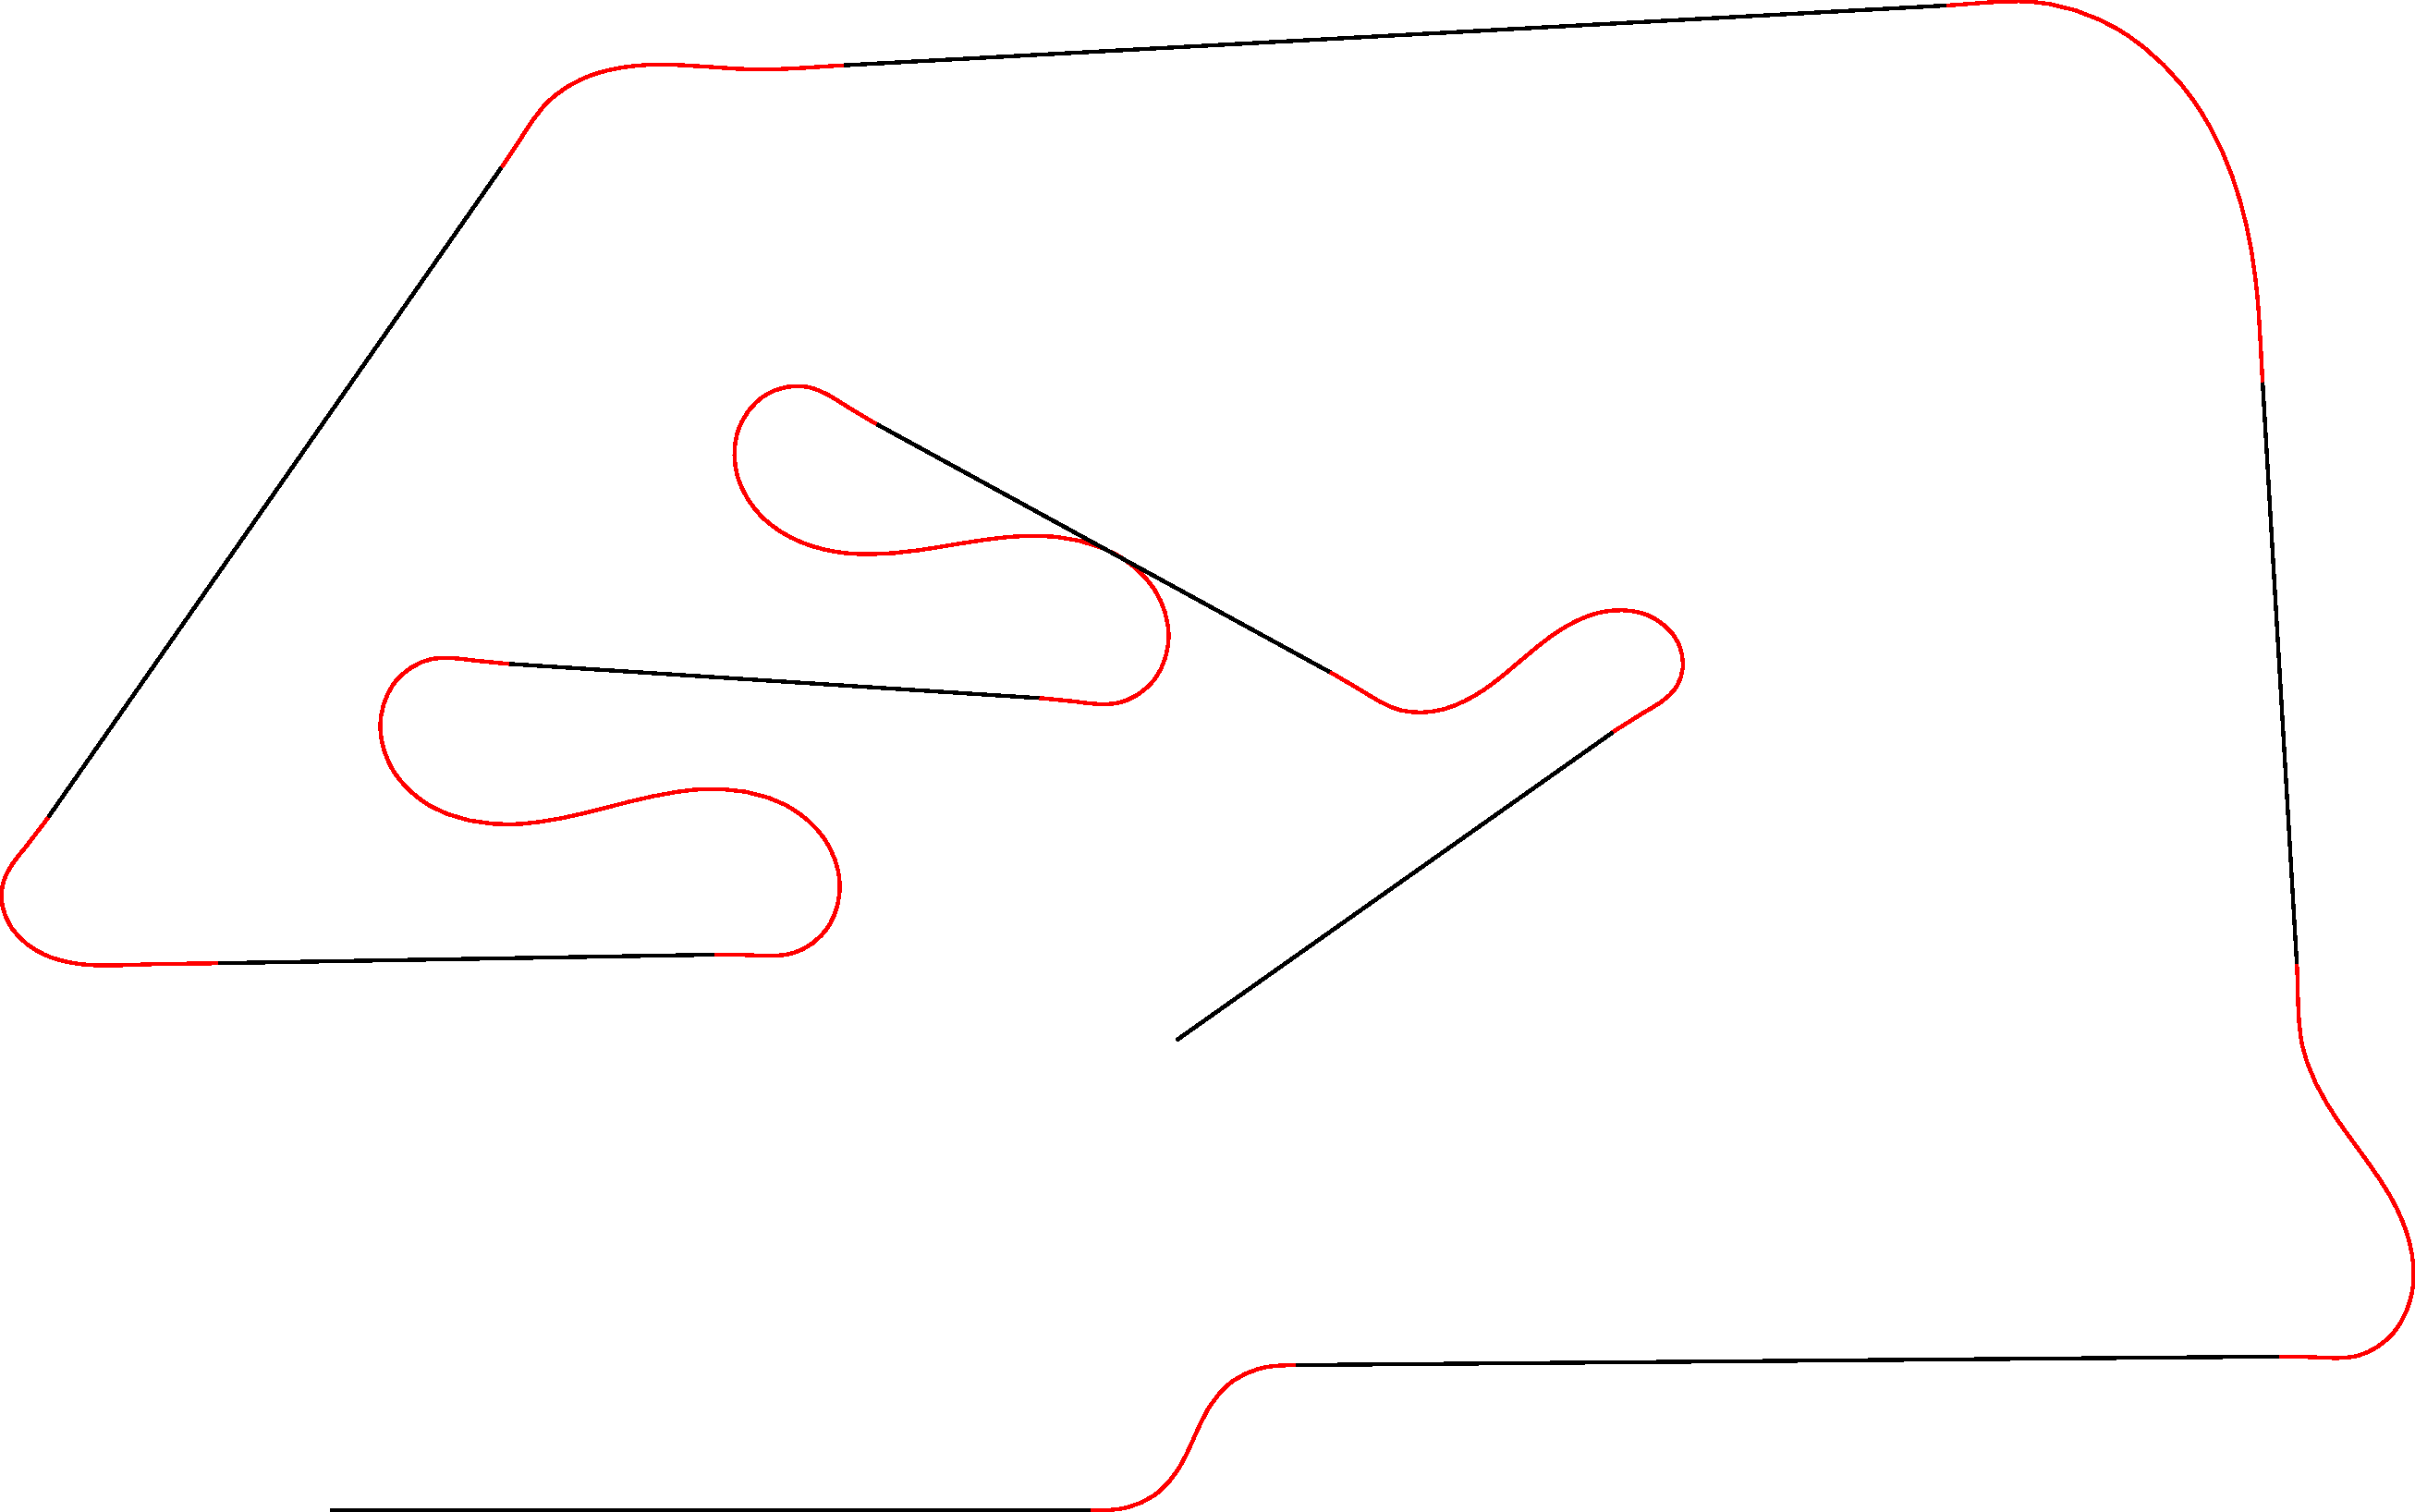
\includegraphics[width=\textwidth]{images/smooth/smooth_connections_1.pdf}
\caption{Various random lines with generated connection}
\end{subfigure}
\par \bigskip

\begin{subfigure}[b]{0.45\textwidth}
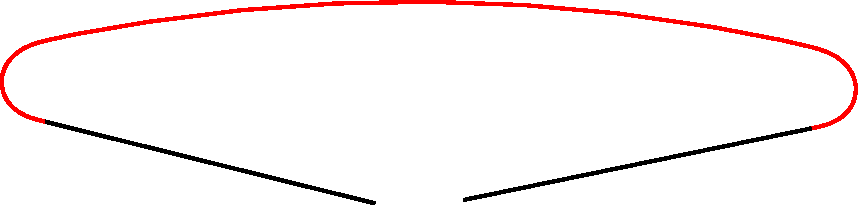
\includegraphics[width=\textwidth]{images/smooth/smooth_connections_2.pdf}
\caption{Highlighting the generated solution to the infinite arc problem}
\end{subfigure}
~
\begin{subfigure}[b]{0.45\textwidth}
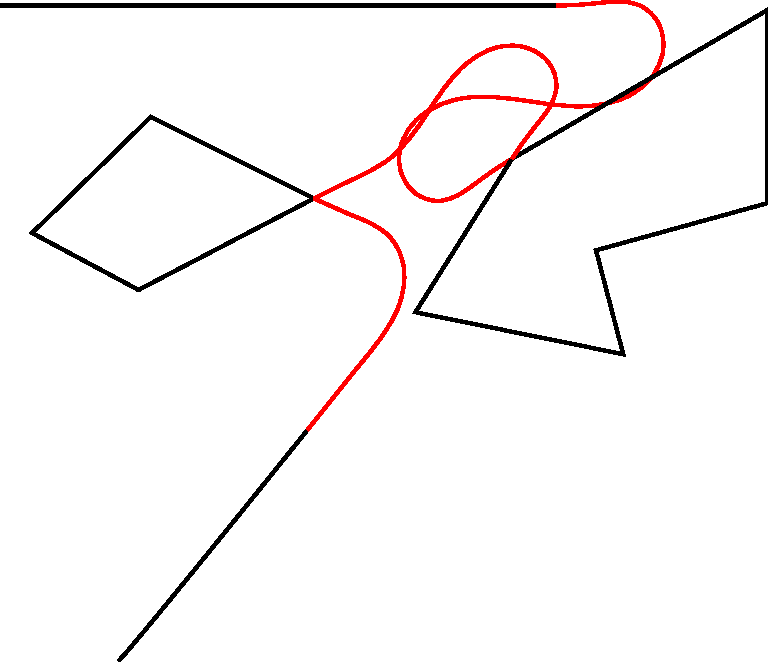
\includegraphics[width=\textwidth]{images/smooth/smooth_connections_3.pdf}
\caption{Connecting random lines and polygons}
\end{subfigure}

\caption{Smooth connections as obtained by applying the heuristic}
\end{figure}
